\documentclass[tikz, border=10pt]{standalone}
\usetikzlibrary{shapes, arrows, positioning, fit, calc}

\begin{document}
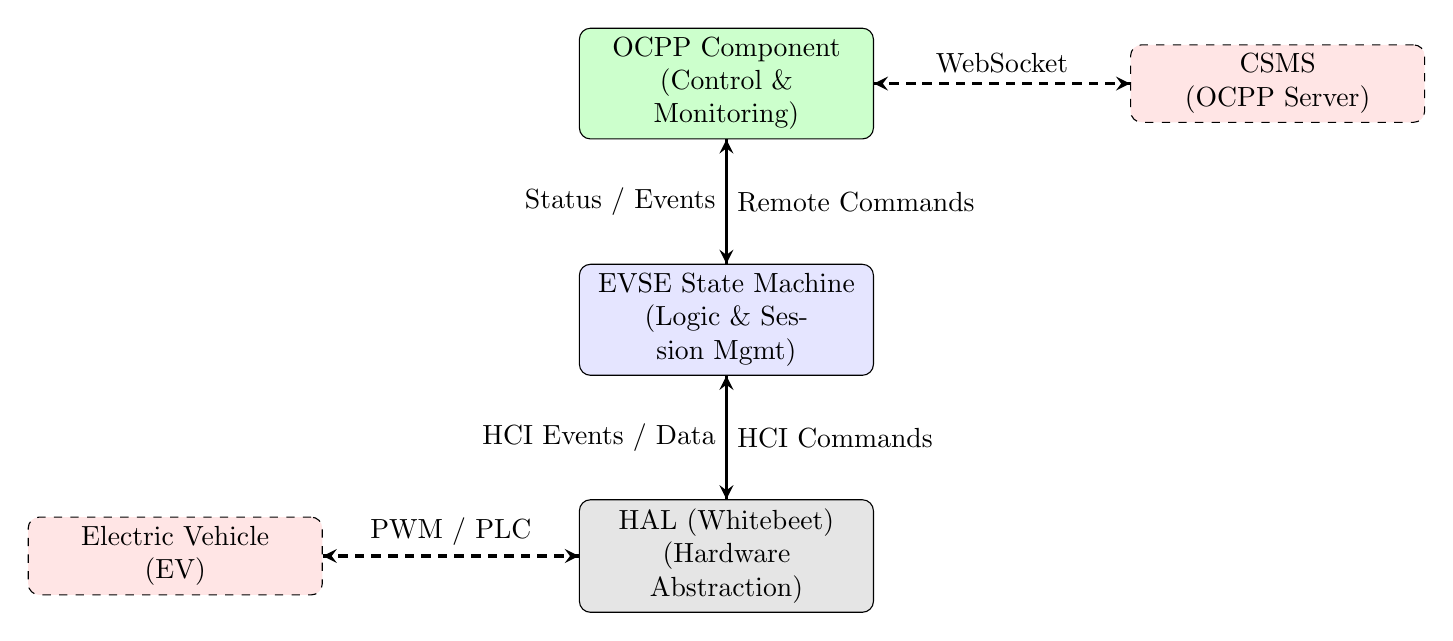
\begin{tikzpicture}[
    node distance=2cm, 
    auto,
    >=stealth,
    block/.style={rectangle, draw, fill=blue!10, text width=3.5cm, text centered, rounded corners, minimum height=1.5em},
    line/.style={draw, ->, very thick},
    dashed_box/.style={draw, dashed, inner sep=0.5cm, label={[anchor=north west]north west:#1}}
]

    % Nodes
    \node [block, fill=green!20] (ocpp) {OCPP Component \\ (Control \& Monitoring)};

    \node [block, dashed, fill=red!10, right of=ocpp, node distance=7cm] (csms) {CSMS \\ (OCPP Server)};
    
    \node [block, below of=ocpp, node distance=3cm] (evse) {EVSE State Machine \\ (Logic \& Session Mgmt)};
    
    \node [block, below of=evse, node distance=3cm, fill=gray!20] (hal) {HAL (Whitebeet) \\ (Hardware Abstraction)};

    \node [block, dashed, fill=red!10, left of=hal, node distance=7cm] (ev) {Electric Vehicle \\ (EV)};

    % Connections
    \path [line, dashed] (csms) -- node [above] {WebSocket} (ocpp);
    \path [line, dashed] (ocpp) -- (csms);

    \path [line] (ocpp) -- node [right] {Remote Commands} (evse);
    \path [line] (evse) -- node [left] {Status / Events} (ocpp);

    \path [line] (evse) -- node [right] {HCI Commands} (hal);
    \path [line] (hal) -- node [left] {HCI Events / Data} (evse);

    \path [line, dashed] (hal) -- node [above] {PWM / PLC} (ev);
    \path [line, dashed] (ev) -- (hal);

    % Optional: Grouping or Labels
    % \node [draw=red, fit=(ocpp) (evse) (hal), inner sep=0.5cm, dashed] {};

\end{tikzpicture}
\end{document}
